\documentclass[10pt, a4paper, twocolumn]{article}

\usepackage[utf8]{inputenc}
\usepackage[T1]{fontenc}
\usepackage{lmodern}
\usepackage[main=turkish,provide=*]{babel}
\usepackage[margin=2cm]{geometry}
\usepackage{parskip}
\usepackage{caption}
\usepackage{enumitem}
\setlist{nosep, leftmargin=*}
\usepackage{graphicx}
\graphicspath{{figures/}}

\usepackage[dvipsnames]{xcolor}
\usepackage[colorlinks=true,
            linkcolor=NavyBlue,
            citecolor=ForestGreen,
            urlcolor=BrickRed]{hyperref}

\usepackage{amsmath}
\usepackage{amssymb}
\usepackage{tikz}
\usetikzlibrary{positioning,arrows.meta,babel}
\usepackage{listings}
\lstset{
  basicstyle=\ttfamily\small,
  keywordstyle=\color{NavyBlue}\bfseries,
  commentstyle=\color{Gray},
  stringstyle=\color{BrickRed},
  breaklines=true,
  frame=single,
  framesep=4pt,
  xleftmargin=8pt,
  xrightmargin=8pt,
  numbers=left,
  numberstyle=\tiny\color{Gray},
  tabsize=2,
  showstringspaces=false
}

\lstdefinelanguage{turtle}{
  morekeywords={@prefix, a, owl:Class, owl:ObjectProperty, owl:DatatypeProperty,
                rdfs:subClassOf, rdfs:domain, rdfs:range, rdfs:label, rdfs:comment,
                owl:Ontology, rdf:type, owl:NamedIndividual},
  sensitive=true,
  morecomment=[l]{\#},
  morestring=[b]",
}

\lstdefinelanguage{sparql}{
  morekeywords={PREFIX, SELECT, WHERE, FILTER, OPTIONAL, ORDER, BY, IN,
                DISTINCT, UNION, GROUP, COUNT, AS, ASK, CONSTRUCT, FROM},
  sensitive=true,
  morecomment=[l]{\#},
  morestring=[b]",
}


\title{%
  \textbf{BDM Tabanlı Etmen Sistemleri Ontolojisi}
}

\author{
  Sami Tugal\\
  \texttt{91240000386@ogrenci.ege.edu.tr}\\
  Ege Üniversitesi Bilgisayar Mühendisliği Bölümü\\
  ORCID: 0009-0008-6595-7053
  \and
  Prof. Dr. Murat Osman Ünalır\\
  Ege Üniversitesi Bilgisayar Mühendisliği Bölümü\\
  ORCID: 0000-0003-4531-0566
}

\date{\today}

\renewcommand{\abstractname}{Özet}

\begin{document}
\maketitle

\begin{abstract}
    Son yıllarda büyük dil modeli (BDM) tabanlı etmenlerin yaygınlaşmasıyla birlikte LangChain, AutoGen ve CrewAI gibi çerçeveler benzer kavramları farklı isim ve soyutlamalarla sunmakta; alanda ortak, çerçeveden bağımsız ve biçimsel olarak doğrulanabilir bir kavramsal model bulunmamaktadır. Bu çalışma, BDM tabanlı etmen sistemleri için OWL~2 tabanlı bir ontoloji önermektedir. Ontoloji; etmen çekirdeği, araç kullanımı, hafıza, oturum ve mesaj akışı, model yapılandırması ile çok-etmenli orkestrasyon olmak üzere altı katmanda 47 sınıf, 51 nesne özelliği ve 79 veri özelliği içermekte ve OASIS~2 temel ontolojisini terminolojik referans olarak yeniden kullanmaktadır. Tasarım üç bağımsız yöntemle doğrulanmıştır: (i) HermiT reasoner ile tutarlılık denetimi ve tanımlı sınıflar üzerinde otomatik sınıflandırma (örn.\ \texttt{CodeExecutorAgent} bireyinin \texttt{AutonomousAgent} ve \texttt{MemoryAugmentedAgent} olarak çıkarsanması), (ii) Giriş'te tanımlanan altı yetkinlik sorusunun SPARQL~1.1 sorgularıyla yanıtlanması ve (iii) OOPS! aracıyla tasarım kalitesi taraması (\textit{Critical} tuzak: 0). Ayrıca ontolojinin çerçeveden bağımsızlık iddiası, LangChain ve CrewAI çerçevelerinin gerçek sınıf hiyerarşilerinin canlı \emph{reflection} ile çıkarılıp 37 ontoloji terimine eşlenmesiyle ampirik olarak sınanmıştır. Tüm artefaktlar (OWL dosyaları, SPARQL sorguları ve üretici betikler) açık biçimde paylaşılmaktadır.
\end{abstract}

\section{Giriş}

Büyük dil modelleri (BDM), yapay zeka alanında son yıllarda hızla gelişen ve yaygınlaşan bir teknolojidir. Doğal dil işleme, görüntü işleme ve ses işleme gibi pek çok alanda önemli başarılar elde eden bu modeller, uygun bileşenlerle birleştirildiğinde etmen tabanlı sistemlerin temelini oluşturmaktadır~\cite{xi2025rise}. Bu çalışmada geliştirilen ontoloji; söz konusu bileşenleri, aralarındaki ilişkileri, karakteristik özelliklerini ve bir araya gelerek oluşturdukları etmen yapısını sistematik biçimde modellemektedir.

Ontoloji, BDM tabanlı etmen sistemlerinin kavramsal yapısını herhangi bir çerçeveden bağımsız olarak ele almakta ve aşağıdaki temel bileşenleri kapsamaktadır:

\begin{itemize}
    \item Etmen çekirdeği ve rolü
    \item Araç (tool) ilişkileri
    \item Hafıza mekanizmaları
    \item Oturum ve mesaj akışı
    \item Çok-etmenli koordinasyon yapıları
\end{itemize}

Öte yandan aşağıdaki konular kapsam dışında bırakılmıştır:

\begin{itemize}
    \item Transformer tabanlı modellerin eğitim süreci
    \item Donanım altyapısı
    \item Kullanıcı arayüzü tasarımı
    \item Çerçeveye özgü implementasyon detayları
\end{itemize}

Mevcut literatürde BDM tabanlı etmen sistemleri için genel kabul görmüş, çerçeve bağımsız bir meta-model bulunmamaktadır. LangChain, AutoGen~\cite{wu2024autogen} ve CrewAI gibi farklı çerçeveler, benzer kavramları farklı isim ve soyutlamalarla sunmaktadır. Bu ontoloji, söz konusu boşluğu kapatarak etmen tasarımına ilişkin ortak bir kavramsal zemin oluşturmayı amaçlamaktadır.

Ontolojinin kapsamını ve yeterliliğini doğrulamak üzere aşağıdaki yetkinlik soruları tanımlanmıştır:

\begin{itemize}
    \item Bir etmen hangi araçlara erişebilir ve bu araçların parametrik kısıtları nelerdir?
    \item Bir etmen orchestrator, worker ya da her iki rolde birden mi çalışmaktadır?
    \item Hangi hafıza mekanizmaları hangi etmen tipleriyle ilişkilendirilebilir?
    \item İki etmen arasında görev devri (delegation) hangi koşullarda gerçekleşebilir?
    \item Bir oturum içinde üretilen mesajlar hangi etmene, role ve zaman noktasına aittir?
    \item Çok-etmenli bir grupta koordinasyon nasıl sağlanır?
\end{itemize}

Ontolojinin birincil hedef kitlesi şu gruplardan oluşmaktadır:

\begin{itemize}
    \item \textbf{Yazılım mühendisleri:} Etmen tabanlı sistemleri tasarlayan ve geliştiren kişiler.
    \item \textbf{Alan uzmanları:} BDM tabanlı etmen sistemlerini araştıran akademisyenler ve pratisyenler.
    \item \textbf{Bilgi mühendisleri:} Ontoloji tabanlı akıl yürütme sistemleri geliştiren uzmanlar.
\end{itemize}


\section{Mevcut Ontolojilerin İncelenmesi ve Temel Terimlerin Belirlenmesi}

\subsection{Literatür Taraması}
Ontoloji geliştirme sürecinin bu aşamasında, öncelikle etmen sistemleri alanındaki mevcut ontolojiler incelenerek yeniden kullanım potansiyeli değerlendirilmiş, ardından ontolojide yer alacak temel terimler belirlenmiştir. Anlamsal Web vizyonu çerçevesinde, yazılım etmenlerinin insan adına bilgi sorgulayıp işleyebilmesi için makine tarafından okunabilir ve anlamsal açıdan zengin veri temsillerine ihtiyaç duyulmaktadır. Bu bağlamda W3C tarafından standartlaştırılan Web Ontology Language (OWL~2)~\cite{w3c2012owl2}, Anlamsal Web ontolojilerinin temsili için temel dil olarak kabul görmektedir.

Yapılan literatür taramasında, mevcut ontolojilerin büyük çoğunluğunun klasik çok-etmenli sistem (MAS) mimarilerini modellediği ya da IoT, blockchain gibi belirli bir uygulama alanına özgü kısıtlamalar içerdiği görülmüştür. BDM tabanlı etmen sistemleri alanında 2024--2026 döneminde çeşitli kavramsal modeller ve birleşik taksonomiler (perception/brain/planning/action/tool-use/collaboration eksenleri) önerilmiş; iş süreçleri ve kurumsal iş akışı odaklı endüstriyel çerçeveler de (örn.\ Skan~AI'nin \textit{Agentic Ontology of Work}'ü~\cite{skan2026aow}) ortaya çıkmıştır. Akademik tarafta, ESWC~2026'da sunulan \textit{AgentO}~\cite{agento}, agentic AI sistemlerini etmen (\texttt{Agent}), görev (\texttt{Task}), hedef (\texttt{Goal}), iş akışı deseni (\texttt{WorkflowPattern}/\texttt{WorkflowStep}), takım (\texttt{Team}) ve kaynak bağımlılıkları üzerinden modelleyen 15 sınıflık bir OWL/RDF ontolojisidir; LLM-güdümlü bir çıkarım süreciyle dört çerçeveden (AutoGen, CrewAI, LangGraph, Mastra~AI) 66 agentic iş akışını bilgi grafiğine \emph{örnek} (instance) düzeyinde aktararak değerlendirilmiştir. Bu çalışma ile AgentO birbirini tamamlayıcıdır ancak yöntem ve odak bakımından ayrışır: (i)~\textbf{Yöntem} --- AgentO iş akışlarını LLM ile örnek düzeyinde aktarırken, bu çalışma çerçevelerin sınıf hiyerarşilerini deterministik \emph{reflection} (\texttt{\_\_mro\_\_}) ile \emph{şema} düzeyinde eşleyerek terim karşılıklarını kanıtlar; (ii)~\textbf{Odak} --- AgentO iş akışı ve agentic-pattern düzeyinde kalırken, bu çalışma hafızayı dört alt türe ($\textit{Short}/\textit{Long}/\textit{Episodic}/\textit{Semantic}$) ve stratejilere ayırarak, ayrıca oturum--mesaj akışını, araç çağrı--sonuç zincirini, model yapılandırmasını ve asimetrik/yansımasız \texttt{Delegation} ilişkisini birinci-sınıf tutarak etmenin iç mimarisine iner; (iii)~\textbf{Temel ontoloji ve yeniden kullanım} --- bu çalışma OASIS~2'yi \texttt{owl:imports} ile içe aktarıp \texttt{Agent}~$\sqsubseteq$~\texttt{oasis2:Agent}, \texttt{Capability}~$\sqsubseteq$~\texttt{oasis2:Behaviour} ve \texttt{Task}~$\sqsubseteq$~\texttt{oasis2:TaskDescription} hizalamalarıyla genişletir ve tanımlı sınıflar üzerinde reasoner sınıflandırması yürütür. Bu davranış, Noy ve McGuinness'in \textit{Ontology Development 101} metodolojisinde mevcut ontolojileri ``geliştir ve genişlet'' (\textit{refine and extend}) etmeyi öğütleyen ve birlikte-çalışabilirlik gerektiğinde bunu bir gereklilik olarak niteleyen Adım~2 ilkesiyle birebir örtüşür~\cite{noy2001ontology101}; AgentO ise 15 sınıfının tümünü herhangi bir temel/dış ontolojiyi miras almadan sıfırdan tanımlayarak söz konusu yeniden-kullanım adımını uygulamamaktadır. AgentO buna karşın daha geniş çerçeve kapsamına (dört çerçeve) ve kalıcı IRI altında yayımlanmış bir kaynak altyapısına sahiptir. Bununla birlikte mevcut çalışmaların çoğu ya informal taksonomi ya da iş-akışı/agentic-pattern düzeyinde kalmakta; hafıza katmanlaması, oturum--mesaj akışı ve araç çağrı zincirini birinci-sınıf ve reasoner-doğrulanabilir biçimde, OASIS~2 gibi bir temel ontolojiyle hizalı olarak bir araya getiren çerçeveden bağımsız bir BDM etmen ontolojisi henüz yaygın değildir. Bu çalışma söz konusu kesişimi hedeflemekte ve ayrıca canlı \emph{reflection} ile ampirik kapsama doğrulaması sunarak farklılaşmaktadır. BDM etmenlerini karakterize eden \textit{reasoning-acting} döngüsü~\cite{yao2023react}, dış araç çağırma yeteneği~\cite{schick2023toolformer} ve hafıza katmanı~\cite{packer2023memgpt} gibi temel mekanizmalar, mevcut formal etmen ontolojilerinde doğrudan kavramsal karşılığa sahip değildir.

\textbf{FIPA Standartları:} Foundation for Intelligent Physical Agents \cite{fipa2002acl} tarafından geliştirilen Agent Communication Language (ACL), çok-etmenli sistemlerde iletişim standardı olarak öne çıkmaktadır. FIPA-ACL, mesaj yapısını \textit{performative} (iletişimsel eylem tipi), \textit{sender}, \textit{receiver} ve \textit{content} parametreleri üzerinden tanımlar;
bu standartlarla beraber tanımlanan ACL Performatif, Directory Facilitator kavramları günümüzdeki BDM tabanlı sistemler için geçerli olmakla birlikte, BDM tabanlı sistemlerin gerektirdiği \texttt{Memory}, \texttt{Tool} ve \texttt{Session} kavramlarını içermemektedir.

İncelenen çalışmalar arasında en kapsamlı aday olan OASIS 2 \cite{bella2023oasis2}, OWL 2 tabanlı bir temel ontoloji olup davranışçı (behaviouristic) bir yaklaşım benimsemektedir. Etmenleri dört temel sınıf üzerinden modellemektedir:

\begin{itemize}
    \item \texttt{Agent}: Tüm etmen bireylerini kapsayan temel sınıf; \texttt{hasBehaviour} özelliği ile davranışlara bağlanır.
    \item \texttt{Behaviour}: Etmenin ulaşabileceği hedefleri toplayan yapı; \texttt{consistsOfGoalDescription} özelliği ile hedeflere bağlanır.
    \item \texttt{GoalDescription}: Etmenin gerçekleştirebileceği görevleri içeren hedef tanımları; \texttt{dependsOn} özelliği ile bağımlılık ilişkilerini ifade eder.
    \item \texttt{TaskDescription}: Etmenlerin gerçekleştirdiği atomik operasyonları tanımlayan sınıf.
\end{itemize}

OASIS 2, etmen davranışlarının anlamsal temsilini sağlamakta ve etmenlerin tak-çıkart biçiminde işbirlikçi ortamlara katılmasını mümkün kılmaktadır. Ancak blockchain ve IoT bağlamına özgü kısıtlamalar içermesi ve BDM tabanlı sistemler için kritik olan \texttt{Session}, \texttt{Memory} ve \texttt{Tool} katmanlarını kapsamaması nedeniyle doğrudan içe aktarılması uygun görülmemiştir. Bu değerlendirmeler doğrultusunda ontoloji sıfırdan geliştirilecek; OASIS 2 bünyesindeki \texttt{Agent} ve \texttt{Task} sınıflarının kavramsal tanımları ile FIPA standartlarındaki iletişim protokolleri yalnızca terminolojik referans olarak ele alınacaktır.

İncelenen yaklaşımların BDM tabanlı etmen sistemleri açısından kapsama düzeyi Tablo~\ref{tab:comparison}'de özetlenmiştir. Tablo, hiçbir mevcut yaklaşımın hafıza, araç kullanımı, oturum yönetimi ve orkestrasyon katmanlarını aynı anda OWL~2 tabanlı ve reasoner-doğrulanabilir biçimde, çerçeveden bağımsız olarak kapsamadığını; bu çalışmanın hedeflediği boşluğun bu kesişimde yer aldığını göstermektedir.

\begin{table*}[t]
\centering
\scriptsize
\setlength{\tabcolsep}{4pt}
\renewcommand{\arraystretch}{1.2}
\begin{tabular}{|l|c|c|c|c|c|c|}
\hline
\textbf{Ontoloji / Yaklaşım} & \textbf{Hafıza} & \textbf{Araç} & \textbf{Oturum} & \textbf{Orkestrasyon /} & \textbf{OWL~2 +} & \textbf{Çerçeve/Alan} \\
 & & & & \textbf{Delegasyon} & \textbf{Reasoner} & \textbf{bağımsız} \\
\hline
FIPA-ACL~\cite{fipa2002acl} & -- & -- & -- & K & -- & \checkmark \\
\hline
OASIS~2~\cite{bella2023oasis2} & -- & -- & -- & K & \checkmark & K \\
\hline
Klasik MAS ontolojileri & -- & -- & -- & \checkmark & K & \checkmark \\
\hline
BDM etmen taksonomileri~\cite{sapkota2025taxonomy} & \checkmark & \checkmark & K & \checkmark & -- & \checkmark \\
\hline
AgentO~\cite{agento} & K & \checkmark & -- & \checkmark & \checkmark & \checkmark \\
\hline
\textbf{Bu çalışma} & \checkmark & \checkmark & \checkmark & \checkmark & \checkmark & \checkmark \\
\hline
\end{tabular}
\caption{Mevcut yaklaşımların BDM-etmen kavramları açısından karşılaştırılması (\checkmark: tam kapsam, K: kısmi / dolaylı, --: yok). AgentO tek bir \texttt{Memory} sınıfı içerir (hafıza alt türleri yoktur) ve iş akışı/agentic-pattern modellemesine odaklanır; satır, yayımlanmış tanım ve kamuya açık ontoloji deposuna göre değerlendirilmiştir. OASIS~2 çerçeveden bağımsız bir temel ontolojidir; ancak blockchain/IoT alanına özgü kısıtlar içerdiğinden alan-bağımsızlık açısından kısmi (K) değerlendirilmiştir.}
\label{tab:comparison}
\end{table*}

\subsection{Önemli Terimlerin Belirlenmesi}
Mevcut ontolojilerin yetersiz kaldığı noktalar belirlendikten sonra, ontolojide ifade edilmesi hedeflenen kavramlar sınıf ve slot ayrımı gözetilmeksizin listelenmiştir \cite{noy2001ontology101}. Toplam 37 terim altı grupta sunulmaktadır:

\textbf{Çekirdek Varlıklar:}
\begin{itemize}
    \item \texttt{Agent}: Karar veren, yönlendiren ve diğer bileşenleri orkestre eden temel varlık.
    \item \texttt{AgentGroup}: Ortak bir amaç doğrultusunda birlikte çalışan etmenlerin mantıksal organizasyonu.
    \item \texttt{AgentTemplate}: Somut bir etmen örneği oluşturmak için kullanılan soyut yapılandırma şablonu.
    \item \texttt{Role}: Bir etmenin sistem içindeki işlevsel konumunu ve sorumluluğunu belirleyen tanım.
    \item \texttt{Policy}: Etmenin karar ve davranışlarını kısıtlayan veya yönlendiren kurallar bütünü.
\end{itemize}

\textbf{Etkileşim ve Akış:}
\begin{itemize}
    \item \texttt{Session}: Bir kullanıcı ile etmen arasındaki belirli bir etkileşim sürecini kapsayan bağlam birimi.
    \item \texttt{Message}: Kullanıcıdan ya da etmenden gelen, role ve sıraya sahip tekil iletişim birimi.
    \item \texttt{Observation}: Bir oturum sırasında üretilen token kullanımı, gecikme ve hata gibi sistem düzeyindeki ölçüm kayıtları.
    \item \texttt{Context}: Etmenin karar üretirken değerlendirdiği anlık bağlam penceresi.
\end{itemize}

\textbf{Yetenek Katmanı:}
\begin{itemize}
    \item \texttt{Tool}: Etmen tarafından çağrılabilen, tanımlı bir işi yerine getiren dışsal fonksiyon veya sistem bileşeni.
    \item \texttt{ToolCall}: Etmenin bir aracı belirli parametrelerle çağırma eylemi.
    \item \texttt{ToolResult}: Bir araç çağrısının ürettiği çıktı ya da hata durumu.
    \item \texttt{Resource}: Etmenin erişebildiği dosya, veritabanı veya harici servis gibi veri kaynakları.
    \item \texttt{Action}: Etmenin bir karar sonucunda gerçekleştirdiği somut işlem.
    \item \texttt{Capability}: Bir etmenin sahip olduğu yetenek kümesinin soyut tanımı.
\end{itemize}

\textbf{Hafıza Katmanı:}
\begin{itemize}
    \item \texttt{Memory}: Etmenin geçmiş etkileşimlere ve bilgiye erişimini sağlayan genel hafıza altyapısı.
    \item \texttt{ShortTermMemory}: Aktif oturum süresince geçerli olan kısa vadeli bağlam hafızası.
    \item \texttt{LongTermMemory}: Oturumlar arasında kalıcı olarak saklanan uzun vadeli bilgi deposu.
    \item \texttt{EpisodicMemory}: Geçmiş etkileşimlere ait olaysal kayıtları saklayan hafıza türü.
    \item \texttt{SemanticMemory}: Alan bilgisi ve olgusal bilgiyi temsil eden yapılandırılmış bilgi tabanı.
    \item \texttt{MemoryStrategy}: Hangi bilginin ne zaman saklanacağını ve geri çağrılacağını belirleyen strateji.
\end{itemize}

\textbf{Model ve Yapılandırma:}
\begin{itemize}
    \item \texttt{LLMModel}: Etmenin çıktı üretmek için kullandığı büyük dil modeli.
    \item \texttt{Prompt}: Modele gönderilen ve davranışı yönlendiren girdi metni.
    \item \texttt{SystemPrompt}: Etmenin genel davranışını, rolünü ve kısıtlamalarını tanımlayan sabit yönerge.
    \item \texttt{UserPrompt}: Kullanıcı ya da çağıran sistem tarafından sağlanan, etmene yönlendirilen anlık talep veya soru.
    \item \texttt{PromptTemplate}: Dinamik değişkenler içeren ve çalışma zamanında doldurulabilen prompt şablonu.
    \item \texttt{Parameter}: Modelin sıcaklık ve maksimum token gibi çalışma zamanı ayarlarını tanımlayan değer.
    \item \texttt{ModelConfiguration}: Bir etmen için kullanılacak modeli ve parametrelerini bir arada tanımlayan yapılandırma nesnesi.
\end{itemize}

\textbf{Orkestrasyon ve İletişim:}
\begin{itemize}
    \item \texttt{Task}: Etmenin tamamlaması beklenen, tanımlı giriş ve çıkışa sahip iş birimi.
    \item \texttt{Subtask}: Bir görevin daha küçük ve bağımsız olarak yürütülebilir alt parçası.
    \item \texttt{Plan}: Bir görevi tamamlamak için belirlenen sıralı adımlar dizisi.
    \item \texttt{Workflow}: Birden fazla etmen veya araçın koordineli biçimde yürüttüğü süreç akışı.
    \item \texttt{Delegation}: Bir etmenin görevi başka bir etmene devretme ilişkisi.
    \item \texttt{ExecutionContext}: Bir görevin çalıştırıldığı ortam bilgisini ve durumunu kapsayan bağlam nesnesi.
    \item \texttt{Channel}: Etmenler veya etmen ile kullanıcı arasındaki iletişim kanalının soyut tanımı.
    \item \texttt{Protocol}: Etmenler arası mesaj alışverişini düzenleyen iletişim kuralları bütünü.
    \item \texttt{MessageRole}: Bir mesajın sistemdeki rolünü belirleyen etiket (\texttt{user}, \texttt{assistant}, \texttt{system} vb.).
\end{itemize}

Toplam 37 terim belirlenmiştir. Bu terimlerin bir kısmı ilerleyen aşamalarda bağımsız sınıflar olarak tanımlanacak, bir kısmı ise sınıflara ait slot ya da facet olarak modellenecektir.

\section{Ontoloji Tasarımı}

Bu bölümde ontolojinin sınıf hiyerarşisi, nesne ve veri özellikleri, kısıtlar ve bireyler ele alınmaktadır. OWL~2 implementasyonu \texttt{RDF/XML} formatında sunulmaktadır.

\subsection{Sınıf Hiyerarşisi}

Ontoloji 37 terimi altı katmanda organize etmektedir. Her katman işlevsel bir sorumluluğa karşılık gelir.

\medskip
\noindent\textbf{1. Çekirdek Varlıklar}

\begin{itemize}
\item \texttt{Agent} $\sqsubseteq$ \texttt{oasis:Agent}
\item \texttt{AgentGroup}, \texttt{AgentTemplate}
\item \texttt{Role}, \texttt{Policy}
\item \texttt{ModelConfiguration}
\end{itemize}

\noindent\textbf{2. Etkileşim ve Akış}

\begin{itemize}
\item \texttt{Session}, \texttt{Context}, \texttt{Observation}
\item \texttt{Message} $\sqsupset$ \texttt{AgentMessage}, \texttt{UserMessage}
\item \texttt{MessageRole} (oneOf: \texttt{User}, \texttt{Assistant}, \texttt{System}, \texttt{ToolRole})
\end{itemize}

\noindent\textbf{3. Yetenek Katmanı}

\begin{itemize}
\item \texttt{Capability} $\sqsubseteq$ \texttt{oasis:Behaviour}
\item \texttt{Tool}, \texttt{ToolCall}, \texttt{ToolResult}
\item \texttt{Resource}, \texttt{Action}
\end{itemize}

\noindent\textbf{4. Hafıza Katmanı}

\begin{itemize}
\item \texttt{Memory} $\sqsupset$ \texttt{ShortTermMemory}, \texttt{LongTermMemory},\\ \texttt{EpisodicMemory}, \texttt{SemanticMemory}
\item \texttt{MemoryStrategy} $\sqsupset$ \texttt{CompressionStrategy},\\ \texttt{EvictionStrategy}, \texttt{RetrievalStrategy}
\end{itemize}

\noindent\textbf{5. Model ve Yapılandırma}

\begin{itemize}
\item \texttt{LLMModel}, \texttt{Parameter}
\item \texttt{Prompt} $\sqsupset$ \texttt{SystemPrompt}, \texttt{UserPrompt}
\item \texttt{PromptTemplate}
\end{itemize}

\noindent\textbf{6. Orkestrasyon ve İletişim}

\begin{itemize}
\item \texttt{Task} $\sqsupset$ \texttt{Subtask}; \texttt{Plan}, \texttt{Workflow}
\item \texttt{Delegation}, \texttt{ExecutionContext}
\item \texttt{Channel}, \texttt{Protocol} (örn.\ FIPA-ACL, JSON-RPC, MCP~\cite{anthropic2024mcp})
\end{itemize}

Şekil~\ref{fig:agent-graph}, ontolojinin merkezindeki \texttt{Agent} sınıfının diğer temel sınıflara nesne özellikleri aracılığıyla nasıl bağlandığını özetlemektedir.

\begin{figure*}[t]
\centering
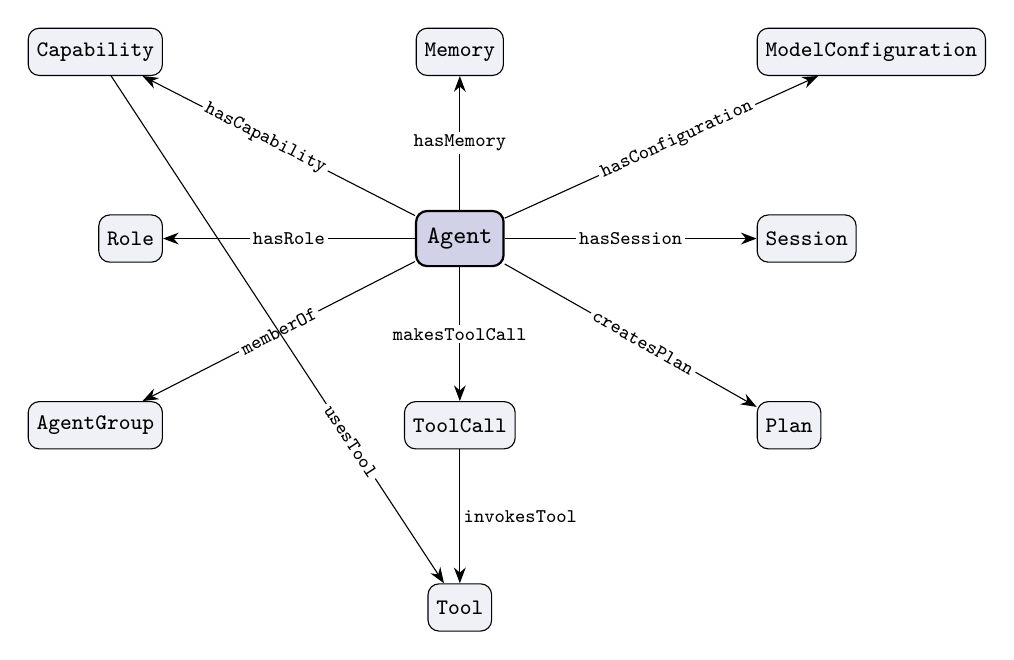
\begin{tikzpicture}[
  >={Stealth[length=2mm]},
  node distance=17mm and 32mm,
  cls/.style={draw, rounded corners, fill=NavyBlue!6, font=\footnotesize\ttfamily,
              minimum height=6mm, inner sep=3pt},
  core/.style={draw, thick, rounded corners, fill=NavyBlue!18, font=\small\ttfamily\bfseries,
               minimum height=7mm, inner sep=4pt},
  rel/.style={->},
  lbl/.style={font=\scriptsize\ttfamily, fill=white, inner sep=1.2pt}
]
\node[core] (agent) {Agent};
\node[cls, above left=of agent]  (cap)     {Capability};
\node[cls, above=of agent]       (mem)     {Memory};
\node[cls, above right=of agent] (cfg)     {ModelConfiguration};
\node[cls, left=of agent]        (role)    {Role};
\node[cls, right=of agent]       (session) {Session};
\node[cls, below left=of agent]  (group)   {AgentGroup};
\node[cls, below=of agent]       (tc)      {ToolCall};
\node[cls, below right=of agent] (plan)    {Plan};
\node[cls, below=of tc]          (tool)    {Tool};

\draw[rel] (agent) -- (cap)     node[lbl, sloped, pos=0.55] {hasCapability};
\draw[rel] (agent) -- (mem)     node[lbl, pos=0.5]          {hasMemory};
\draw[rel] (agent) -- (cfg)     node[lbl, sloped, pos=0.55] {hasConfiguration};
\draw[rel] (agent) -- (role)    node[lbl, pos=0.5]          {hasRole};
\draw[rel] (agent) -- (session) node[lbl, pos=0.5]          {hasSession};
\draw[rel] (agent) -- (group)   node[lbl, sloped, pos=0.5]  {memberOf};
\draw[rel] (agent) -- (tc)      node[lbl, pos=0.5]          {makesToolCall};
\draw[rel] (agent) -- (plan)    node[lbl, sloped, pos=0.55] {createsPlan};
\draw[rel] (tc)    -- (tool)    node[lbl, right, pos=0.5]   {invokesTool};
\draw[rel] (cap)   -- (tool)    node[lbl, sloped, pos=0.72] {usesTool};
\end{tikzpicture}
\caption{\texttt{Agent} sınıfını merkez alan temel nesne özelliği ilişkileri. \texttt{hasConfiguration} \textit{exactly~1}, \texttt{hasCapability} ise \textit{someValuesFrom} kısıtıyla daraltılmıştır.}
\label{fig:agent-graph}
\end{figure*}

\subsection{Tanımlı Sınıflar (Faz~4)}

OWL~2 eşdeğerlik aksiyomuyla üç özelleşmiş etmen tipi türetilmiştir. Bu tanımlar bir reasoner aracılığıyla bireylerin otomatik sınıflandırılmasını sağlar:

\begin{align*}
\textit{AutonomousAgent} &\equiv A \sqcap \exists hM.M \sqcap \exists mTC.TC \\
\textit{MemoryAugmentedAgent} &\equiv A \sqcap \exists hM.LTM \\
\textit{PlanningAgent} &\equiv A \sqcap \exists cP.P \sqcap \lnot(\exists mTC.TC)
\end{align*}

\noindent Kısaltmalar: $A$=\texttt{Agent}, $hM$=\texttt{hasMemory}, $M$=\texttt{Memory}, $mTC$=\texttt{makesToolCall}, $TC$=\texttt{ToolCall}, $LTM$=\texttt{LongTermMemory}, $cP$=\texttt{createsPlan}, $P$=\texttt{Plan}.

Ek olarak iki birleşim (union) sınıfı tanımlanmıştır:
\begin{itemize}
\item \texttt{ExecutableEntity} $\equiv$ \texttt{Task} $\sqcup$ \texttt{Workflow}
\item \texttt{MemoryContent} $\equiv$ \texttt{Message} $\sqcup$ \texttt{Session}
\end{itemize}

\noindent \texttt{MemoryContent}, \texttt{hasMemory} ve hafıza saklama özelliklerinin (\texttt{storesMessage}, \texttt{recordsSession}) ortak range'i olarak işlev görür: hafıza katmanı için \emph{neyin hatırlanabilir bir içerik olduğunu} tek bir tip altında yakalar. Böylece \texttt{Session} bireyleri (oturum-düzeyi epizotlar) ile \texttt{Message} bireyleri (mesaj-düzeyi parçacıklar) farklı granülaritede oldukları halde hafıza sorgularında birlikte ele alınabilir.

Ve kapalı liste (oneOf) ile tanımlı bir çalıştırma modu:
\begin{itemize}
\item \texttt{ExecutionMode} $\equiv$ \{\texttt{Sync}, \texttt{Async}\}
\end{itemize}

\noindent\textbf{Toplam sınıf dökümü.} Ontoloji 47 OWL sınıfı içerir: Bölüm~2.2'deki 37 temel terimin OWL karşılıklarına ek olarak Faz~4'te tanımlanan üç eşdeğerlik sınıfı (\texttt{AutonomousAgent}, \texttt{MemoryAugmentedAgent}, \texttt{PlanningAgent}), iki birleşim sınıfı (\texttt{ExecutableEntity}, \texttt{MemoryContent}), bir oneOf sınıfı (\texttt{ExecutionMode}), \texttt{Message} altında iki alt tip (\texttt{AgentMessage}, \texttt{UserMessage}) ve \texttt{MemoryStrategy} altında üç alt tip (\texttt{Compression-}, \texttt{Eviction-}, \texttt{RetrievalStrategy}) yer alır.

\subsection{Nesne Özellikleri}

Tablo~\ref{tab:all-objprop}, ontolojideki tüm nesne özelliklerini domain, range ve aksiyom bilgisiyle özetlemektedir.

\begin{center}
\tiny
\begin{tabular}{|p{2.1cm}|p{1.4cm}|p{1.4cm}|p{1.5cm}|}
\hline
\textbf{Özellik} & \textbf{Domain} & \textbf{Range} & \textbf{Aksiyom} \\
\hline
\texttt{accessesResource} & Tool & Resource & {-} \\
\hline
\texttt{capabilityOf} & Capability & Agent & inverseOf \\
\hline
\texttt{coordinatesVia} & AgentGroup & Workflow & {-} \\
\hline
\texttt{createsPlan} & Agent & Plan & {-} \\
\hline
\texttt{delegatedBy} & Agent & Delegation & inverseOf \\
\hline
\texttt{delegatedTask} & Delegation & Task & Functional \\
\hline
\texttt{delegatesTo} & Delegation & Agent & Asymm., Irref. \\
\hline
\texttt{delegator} & Delegation & Agent & Functional \\
\hline
\texttt{followsProtocol} & Ch./Del./Wf. & Protocol & {-} \\
\hline
\texttt{forRole} & Prompt & MessageRole & {-} \\
\hline
\texttt{generatedBy} & AgentMsg. & Agent & Functional \\
\hline
\texttt{hasAction} & ToolCall & Action & {-} \\
\hline
\texttt{hasCapability} & Agent & Capability & someValuesFrom \\
\hline
\texttt{hasConfiguration} & Agent & ModelConf. & exactly 1 \\
\hline
\texttt{hasContext} & Agent & Context & {-} \\
\hline
\texttt{hasMember} & AgentGroup & Agent & inverseOf \\
\hline
\texttt{hasMemory} & Agent & Memory & {-} \\
\hline
\texttt{hasMemoryStrategy} & Memory & MemStrategy & {-} \\
\hline
\texttt{hasMessage} & Session & Message & inverseOf \\
\hline
\texttt{hasMessageRole} & Message & MessageRole & Functional \\
\hline
\texttt{hasObservation} & Session & Observation & inverseOf \\
\hline
\texttt{hasParameter} & ModelConf. & Parameter & {-} \\
\hline
\texttt{hasPlan} & Workflow & Plan & {-} \\
\hline
\texttt{hasPolicy} & Agent & Policy & {-} \\
\hline
\texttt{hasPrompt} & ModelConf. & Prompt & {-} \\
\hline
\texttt{hasRole} & Agent & Role & {-} \\
\hline
\texttt{hasSession} & Agent/Group & Session & {-} \\
\hline
\texttt{hasSharedMemory} & AgentGroup & Memory & {-} \\
\hline
\texttt{hasStep} & Plan & Task & allValuesFrom \\
\hline
\texttt{instantiates} & Agent & AgentTemplate & {-} \\
\hline
\texttt{invokedBy} & ToolCall & Agent & {-} \\
\hline
\texttt{invokesTool} & ToolCall & Tool & someValuesFrom \\
\hline
\texttt{madeBy} & Observation & Agent & {-} \\
\hline
\texttt{makesToolCall} & Agent & ToolCall & {-} \\
\hline
\texttt{memberOf} & Agent & AgentGroup & {-} \\
\hline
\texttt{observedIn} & Observation & Session & inverseOf \\
\hline
\texttt{partOfSession} & Message & Session & inverseOf \\
\hline
\texttt{playedBy} & Role & Agent & {-} \\
\hline
\texttt{producesResult} & ToolCall & ToolResult & {-} \\
\hline
\texttt{promptOf} & Prompt & ModelConf. & {-} \\
\hline
\texttt{recordsSession} & EpisodicMem. & Session & {-} \\
\hline
\texttt{resultOf} & ToolResult & ToolCall & Functional \\
\hline
\texttt{runsIn} & Task & ExecutionCtx. & Functional \\
\hline
\texttt{sessionOf} & Session & Ag./AgGr.\,$\sqcup$ & {-} \\
\hline
\texttt{storesMessage} & ShortTermMem. & Message & {-} \\
\hline
\texttt{subtaskOf} & Subtask & Task & Func., Asym., Irref. \\
\hline
\texttt{toolFor} & Tool & Capability & inverseOf \\
\hline
\texttt{triggeredBy} & Delegation & Policy & Functional \\
\hline
\texttt{usesModel} & ModelConf. & LLMModel & {-} \\
\hline
\texttt{usesTool} & Capability & Tool & {-} \\
\hline
\texttt{viaChannel} & Workflow & Channel & {-} \\
\hline
\end{tabular}
\captionof{table}{Tüm nesne özellikleri (51 adet)}
\label{tab:all-objprop}
\end{center}

\subsection{\texttt{Agent} Varlığının Kapsamı}

\texttt{Agent}, ontolojinin merkez sınıfıdır. Sınıf \texttt{oasis:Agent}'tan türetilmiş ve iki zorunlu OWL kısıtıyla daraltılmıştır: her etmen en az bir yeteneğe (\texttt{someValuesFrom hasCapability}) ve tam olarak bir konfigürasyona (\texttt{exactly~1 hasConfiguration}) sahip olmalıdır.

\subsubsection*{Nesne Özellikleri}

\begin{center}
\tiny
\begin{tabular}{|p{2.1cm}|p{1.6cm}|p{2.3cm}|}
\hline
\textbf{Özellik} & \textbf{Yön} & \textbf{Aksiyom / Anlam} \\
\hline
\texttt{hasCapability} & Agent$\to$Capability & someValuesFrom \\
\hline
\texttt{hasConfiguration} & Agent$\to$ModelConf. & exactly 1 \\
\hline
\texttt{hasContext} & Agent$\to$Context & {-} \\
\hline
\texttt{hasMemory} & Agent$\to$Memory & {-} \\
\hline
\texttt{hasPolicy} & Agent$\to$Policy & {-} \\
\hline
\texttt{hasRole} & Agent$\to$Role & {-} \\
\hline
\texttt{hasSession} & Agent$\to$Session & {-} \\
\hline
\texttt{makesToolCall} & Agent$\to$ToolCall & {-} \\
\hline
\texttt{memberOf} & Agent$\to$AgentGroup & {-} \\
\hline
\texttt{createsPlan} & Agent$\to$Plan & {-} \\
\hline
\texttt{delegatedBy} & Agent$\to$Delegation & inverseOf \\
\hline
\texttt{capabilityOf} & Capability$\to$Agent & inverseOf \\
\hline
\texttt{generatedBy} & AgentMsg.$\to$Agent & Functional \\
\hline
\texttt{delegatesTo} & Delegation$\to$Agent & Asymm., Irref. \\
\hline
\texttt{delegator} & Delegation$\to$Agent & Functional \\
\hline
\texttt{hasMember} & AgentGroup$\to$Agent & inverseOf \\
\hline
\end{tabular}
\captionof{table}{\texttt{Agent} nesne özellikleri}
\label{tab:agent-obj}
\end{center}

\subsubsection*{Veri Özellikleri}

\begin{center}
\tiny
\begin{tabular}{|p{2.1cm}|p{1.4cm}|p{2.5cm}|}
\hline
\textbf{Özellik} & \textbf{Tip} & \textbf{Açıklama} \\
\hline
\texttt{agentId} & string & Benzersiz kimlik (Functional) \\
\hline
\texttt{agentName} & string & İnsan okunabilir ad \\
\hline
\texttt{agentVersion} & string & Sürüm etiketi \\
\hline
\texttt{isActive} & boolean & Çalışma durumu \\
\hline
\texttt{createdAt} & dateTime & Oluşturulma zamanı \\
\hline
\end{tabular}
\captionof{table}{\texttt{Agent} veri özellikleri}
\label{tab:agent-data}
\end{center}

\subsubsection*{Ayrıklık Kısıtları}

\texttt{Agent}, \texttt{Memory}, \texttt{Message}, \texttt{Session} ve \texttt{Tool} sınıfları \texttt{owl:AllDisjointClasses} aksiyomuyla birbirinden tamamen ayrılmıştır. Bu kısıt, bir bireyin aynı anda birden fazla temel sınıfa üye olmasını önler.

\subsubsection*{Somut Bireyler}

Çok-etmenli araştırma sistemi senaryosunda dört bireysel etmen örneklenmiştir:

\begin{itemize}
\item \textbf{\texttt{OrchestratorAgent}}: GPT-4o kullanan koordinatör; araştırma oturumunu yönetir.
\item \textbf{\texttt{ResearchPlannerAgent}}: Plan üreten, araç çağrısı yapmayan; reasoner tarafından \texttt{PlanningAgent} olarak çıkarılabilir.
\item \textbf{\texttt{CodeExecutorAgent}}: Uzun vadeli ve epizodik belleğe sahip, araç çağrısı yapan; \texttt{AutonomousAgent} olarak çıkarılabilir.
\item \textbf{\texttt{ReviewerAgent}}: Llama-3 kullanan, dosya okuma yeteneğine sahip değerlendirici etmen.
\end{itemize}

\section{Doğrulama ve Test}

Ontoloji ile birlikte tüm SPARQL sorguları, üretici betikler ve değerlendirme artefaktları kalıcı olarak Zenodo'da arşivlenmiştir (DOI: 10.5281/zenodo.20571344) ve açık bir depoda geliştirilmektedir.\footnote{\url{https://doi.org/10.5281/zenodo.20571344} --- \url{https://github.com/samitugal/ontology-of-llm-based-agentic-ai}} Ontolojinin tasarım aşamasında tanımlanan kavramsal yapının iç tutarlılığı ve Bölüm~1'de belirlenen yetkinlik sorularını yanıtlama kapasitesi, üç ayrı doğrulama yöntemiyle sınanmıştır. İlk yöntemde HermiT reasoner~\cite{glimm2014hermit} aracılığıyla aksiyom kümesinin tutarlılığı kontrol edilmiş ve tanımlı sınıflar üzerinde otomatik sınıflandırma yürütülmüştür. İkinci yöntemde yetkinlik sorularının her biri SPARQL~1.1~\cite{w3c2013sparql} ile sorgulanmış ve elde edilen sonuçlar beklenen sonuçlarla karşılaştırılmıştır. Üçüncü yöntemde ise ontolojinin modelleme kalitesi OOPS! (OntOlogy Pitfall Scanner!)~\cite{poveda2014oops} aracıyla taranmıştır.

\subsection{Reasoner Tutarlılık Kontrolü}

HermiT reasoner, geliştirilen ontolojiyi (76 birey, 47 sınıf, 51 nesne özelliği) OASIS~2 ile birlikte yüklemiş ve tutarlılık analizine tabi tutmuştur. Sonuçlar üç açıdan değerlendirilmektedir:

\begin{itemize}
\item Ontoloji \textbf{tutarlıdır} (\textit{consistent}); hiçbir sınıf \texttt{owl:Nothing} ile eşdeğer olarak çıkarsanmamıştır.
\item \texttt{AllDisjointClasses} aksiyomları (\texttt{Agent}, \texttt{Memory}, \texttt{Message}, \texttt{Session}, \texttt{Tool}) sağlanmış; herhangi bir birey iki ayrık sınıfa eşzamanlı üyelik göstermemektedir.
\item Tanımlı sınıflar üzerinde reasoner, \texttt{CodeExecutorAgent} bireyini hem \texttt{AutonomousAgent} hem \texttt{MemoryAugmentedAgent} olarak otomatik sınıflandırmıştır.
\end{itemize}

\noindent Sınıflandırma sonuçları, ontolojinin Açık Dünya Varsayımına (Open World Assumption, OWA) tabi olduğunu da somut biçimde ortaya koymuştur. Örneğin \texttt{PlanningAgent} tanımı $\textit{Agent} \sqcap \exists \textit{createsPlan}.\textit{Plan} \sqcap \lnot(\exists \textit{makesToolCall}.\textit{ToolCall})$ biçiminde negasyon içermektedir; reasoner, \texttt{ResearchPlannerAgent} bireyinin araç çağrısı yapmadığını ABox kapatılmadığı sürece çıkarsayamamaktadır. Bu davranış bir hata değil, OWA'nın beklenen sonucudur ve ontolojinin doğru biçimde modellendiğine işaret etmektedir.

Bu kapamanın etkisini somut olarak göstermek için ek bir kontrollü deney yürütülmüştür. \texttt{ResearchPlannerAgent} bireyine, araç çağrısı yapmadığını bildiren bir yerel kapama aksiyomu --- OWL Functional sözdiziminde \texttt{Class\-Assertion(Object\-Complement\-Of(Object\-Some\-Values\-From(:makesToolCall :ToolCall)) :Research\-PlannerAgent)} --- eklenmiş ve ontoloji HermiT ile yeniden çıkarıma sokulmuştur. Kapama öncesinde \texttt{PlanningAgent} tanımlı sınıfının hiçbir üyesi çıkarsanamazken (boş sonuç kümesi), kapama sonrasında reasoner \texttt{ResearchPlannerAgent} bireyini beklendiği gibi \texttt{PlanningAgent} olarak sınıflandırmıştır. Bu sonuç hem \texttt{PlanningAgent} tanımının doğruluğunu hem de OWA kaynaklı çıkarsanamama davranışının yerel kapama (\textit{local closed-world}) ile aşılabildiğini doğrulamakta; böylece Faz~4'te tanımlanan üç özelleşmiş etmen tipinin üçü de (\texttt{AutonomousAgent}, \texttt{MemoryAugmentedAgent}, \texttt{PlanningAgent}) çalışır biçimde gösterilmiş olmaktadır.

\subsection{SPARQL ile Yetkinlik Sorusu Doğrulaması}

Bölüm~1'de tanımlanan altı yetkinlik sorusunun her birine karşılık tek bir SPARQL sorgusu hazırlanmış ve reasoner çıkarımlarıyla zenginleştirilmiş ontoloji üzerinde çalıştırılmıştır. Sorguların tamamı ve ham CSV çıktıları Ek~A'da sunulmaktadır; bu bölümde üç temsilî sorgu ön plana çıkarılmaktadır.

\subsubsection*{Sorgu Q1: Araç Erişimi ve Kaynak Bağı}

Birinci yetkinlik sorusu, etmenlerin hangi araçları kullanabildiğini ve bu araçların eriştiği dış kaynakları sorgulamaktadır:

\begin{lstlisting}[language=sparql]
PREFIX : <http://www.ege.edu.tr/cs/ontology/llm-agent#>
SELECT ?agent ?tool ?resource WHERE {
  ?agent a :Agent ;
         :makesToolCall ?call .
  ?call :invokesTool ?tool .
  OPTIONAL { ?tool :accessesResource ?resource . }
}
\end{lstlisting}

\noindent Sorgu, yalnızca araç çağırma yeteneği aktif olarak modellenen \texttt{CodeExecutorAgent} bireyini sonuç kümesine almıştır. \texttt{CodeInterpreterTool} bireyi \texttt{CodeResource}, \texttt{DBResource} ve \texttt{FileResource} kaynaklarına; \texttt{WebSearchTool} bireyi ise \texttt{WebResource} kaynağına erişmektedir.

\subsubsection*{Sorgu Q3: Hafıza ve Etmen Tipi İlişkisi}

Üçüncü yetkinlik sorusu, hafıza mekanizmalarının hangi etmenlerle ilişkilendirildiğini sorgular. Aşağıdaki sorgu, somut etmen bireyleri ile bağlı oldukları dört hafıza türünü listelemektedir:

\begin{lstlisting}[language=sparql]
PREFIX : <http://www.ege.edu.tr/cs/ontology/llm-agent#>
SELECT ?agent ?memoryType WHERE {
  ?agent a :Agent ;
         :hasMemory ?mem .
  ?mem a ?memoryType .
  FILTER(?memoryType IN (:ShortTermMemory,
    :LongTermMemory, :EpisodicMemory, :SemanticMemory))
}
\end{lstlisting}

\noindent Sorgunun ürettiği sonuç şu şekildedir:

\begin{center}
\scriptsize
\begin{tabular}{|p{2.8cm}|p{2.5cm}|}
\hline
\textbf{Etmen} & \textbf{Hafıza Türü} \\
\hline
\texttt{CodeExecutorAgent} & EpisodicMemory \\
\hline
\texttt{CodeExecutorAgent} & LongTermMemory \\
\hline
\texttt{CodeExecutorAgent} & SemanticMemory \\
\hline
\texttt{ResearchPlannerAgent} & ShortTermMemory \\
\hline
\end{tabular}
\captionof{table}{Q3 sorgusu sonucu}
\label{tab:q3-result}
\end{center}

Elde edilen sonuçlar, \texttt{CodeExecutorAgent} bireyinin uzun vadeli, epizodik ve semantik hafızaya sahip olması nedeniyle \texttt{MemoryAugmentedAgent} tanımlı sınıfının koşulunu sağladığını teyit etmektedir.

\subsubsection*{Sorgu Q4: Görev Devri Koşulları}

Dördüncü yetkinlik sorusu, etmenler arasındaki delegasyon yapısını sorgulamaktadır:

\begin{lstlisting}[language=sparql]
PREFIX : <http://www.ege.edu.tr/cs/ontology/llm-agent#>
SELECT ?delegator ?delegatee ?task WHERE {
  ?d a :Delegation ;
     :delegator ?delegator ;
     :delegatesTo ?delegatee ;
     :delegatedTask ?task .
}
\end{lstlisting}

\noindent Sorgu sonucunda iki delegasyon ilişkisi tespit edilmiştir: \texttt{OrchestratorAgent}, \texttt{SummaryTask} görevini \texttt{ReviewerAgent}'a devretmiş; \texttt{ResearchPlannerAgent} ise \texttt{CodeAnalysisTask} görevini \texttt{CodeExecutorAgent}'a aktarmıştır. \texttt{delegatesTo} özelliğinin asimetrik ve yansımasız (\textit{irreflexive}) olarak tanımlanması nedeniyle, hiçbir etmenin kendisine ya da kendisine devreden bir etmene görev devretmesi mümkün değildir.

\subsection{OOPS! ile Tasarım Kalitesi Taraması}

Biçimsel tutarlılığın ötesinde, ontolojinin modelleme kalitesi OOPS! (OntOlogy Pitfall Scanner!)~\cite{poveda2014oops} çevrimiçi aracıyla değerlendirilmiştir. OOPS!, ontolojileri yaygın modelleme tuzakları (\textit{pitfalls}) açısından üç önem düzeyinde (\textit{Critical}, \textit{Important}, \textit{Minor}) inceleyen, reasoner'dan bağımsız bir araçtır; bu yönüyle mantıksal tutarlılık denetimini tasarım kalitesi denetimiyle tamamlar. Tarama, kaynak ontoloji (\texttt{agentic-ontology.rdf}) üzerinde çalıştırılmıştır.

Sonuçlar Tablo~\ref{tab:oops}'da özetlenmektedir. \textbf{Hiçbir \textit{Critical} tuzak tespit edilmemiş; ontoloji taramadan başarıyla geçmiştir.} Raporlanan sınırlı sayıdaki tuzak ya anlam taşımayan (kozmetik) niteliktedir ya da harici import'tan kaynaklanan yan etkilerdir.

\begin{center}
\scriptsize
\setlength{\tabcolsep}{4pt}
\begin{tabular}{|c|c|p{2.7cm}|c|}
\hline
\textbf{Kod} & \textbf{Önem} & \textbf{Pitfall} & \textbf{Eleman} \\
\hline
P11 & Important & Eksik domain/range & 2 \\
\hline
P34 & Important & Tipsiz sınıf & 3 \\
\hline
P08 & Minor & Eksik açıklama (annotation) & 3 \\
\hline
P13 & Minor & Bildirilmemiş ters ilişki & 27 \\
\hline
\end{tabular}
\captionof{table}{OOPS! pitfall tarama sonuçları (\textit{Critical}: 0). P08 ilk taramada 180 öğeyi etkilemekteydi; annotation katmanı eklendikten sonra yalnızca üç OASIS~2 dış öğesi kalmıştır.}
\label{tab:oops}
\end{center}

\noindent Bulguların yorumu:
\begin{itemize}
\item \textbf{P34 (3):} \texttt{oasis:Agent}, \texttt{oasis:Behaviour} ve \texttt{oasis:TaskDescription} sınıflarının tipsiz görünmesi, taramanın OASIS~2 import'unu çözememesinden kaynaklanan bir yan etkidir; ontolojinin kendi kusuru değildir.
\item \textbf{P11 (2):} \texttt{hasDescription} ve \texttt{updatedAt}, birden çok sınıfta kullanılabilmesi için bilinçli olarak domain'i açık bırakılmış jenerik metadata özellikleridir.
\item \textbf{P08 (3):} İlk taramada 47 sınıf, 51 nesne özelliği ve 79 veri özelliği için \texttt{rdfs:label} ile \texttt{rdfs:comment} eksik bulunmuştu (toplam 177 yerel öğe; OOPS! ayrıca üç OASIS~2 sınıfını da raporlayarak sayıyı 180'e taşımıştı). İkinci taramaya kadar tüm 177 yerel öğeye Türkçe açıklama ve İngilizce etiket annotation'ları enjekte edilmiştir; bu işlem \texttt{ontology/add\_annotations.py} betiği ile tekrarlanabilirdir. Kalan üç öğe yine OASIS~2 dış sınıflarıdır ve P34 ile aynı gerekçeye dahildir.
\item \textbf{P13 (27):} Bildirilmemiş ters ilişki önerileridir; heuristik öneri niteliğinde, anlamsal doğruluğu etkilemeyen \textit{Minor} düzeyinde bir tuzaktır. Ontolojide zaten altı \texttt{inverseOf} çifti açıkça tanımlıdır; geri kalan öneriler tek-yönlü modellenmesi tasarımca tercih edilen özellikleri (örn. \texttt{hasConfiguration}, \texttt{hasMessageRole}) işaret etmektedir.
\end{itemize}

\subsection{Doğrulama Özeti}

Altı yetkinlik sorusu, altı SPARQL sorgusuyla doğrulanmış; reasoner tarafından üretilen iki yeni \texttt{rdf:type} aksiyomu (\texttt{CodeExecutorAgent} için \texttt{AutonomousAgent} ve \texttt{MemoryAugmentedAgent}) ABox'a eklenmiştir. OOPS! pitfall taraması ise hiçbir \textit{Critical} tuzak tespit etmeyerek ontolojinin tasarım kalitesini teyit etmiştir. Tüm sorguların ham çıktıları ve ek sınıflandırma raporu sırasıyla Ek~A ve Ek~C'de yer almaktadır. Bu iki yöntemin yanında, ontolojinin çerçeveden bağımsızlık iddiası üçüncü ve ampirik bir doğrulamayla (LangChain ve CrewAI çerçevelerinin gerçek sınıf hiyerarşilerinin ontolojiye eşlenmesiyle) Ek~B'de sınanmıştır.

\section{Sonuç ve Değerlendirme}

Bu çalışmada, BDM tabanlı etmen sistemleri için OWL~2 tabanlı, reasoner-doğrulanabilir ve çerçeveden bağımsız bir biçimsel kavramsal model geliştirilmiştir. Mevcut literatürdeki ontolojiler klasik çok-etmenli sistem mimarilerine veya IoT/blockchain gibi alana özgü senaryolara odaklanmakta; aynı dönemde önerilen taksonomi ve kurumsal iş akışı çerçeveleri ise informal kalmakta ve hafıza, araç kullanımı, oturum yönetimi ile orkestrasyon katmanlarını birinci-sınıf ve reasoner-denetlenebilir biçimde kapsamamaktadır (Tablo~\ref{tab:comparison}). Geliştirilen ontoloji, söz konusu boşluğu doldurarak farklı çerçevelerin ortak bir anlamsal zemin üzerinde karşılaştırılabilmesini ve birlikte çalışabilirliğini sağlamayı hedeflemektedir.

Çalışmanın somut çıktıları şunlardır:

\begin{itemize}
    \item Altı katmanda 47 sınıf, 51 nesne özelliği ve 79 veri özelliği içeren, HermiT ile tutarlılığı doğrulanmış OWL~2 ontolojisi.
    \item Altı yetkinlik sorusunu yanıtlayan ve reasoner-zenginleştirilmiş ontoloji üzerinde çalıştırılan SPARQL sorgu kataloğu (Ek~A).
    \item LangChain ve CrewAI çerçevelerinin gerçek sınıf hiyerarşilerinin canlı reflection ile ontolojiye eşlenmesi (Ek~B).
    \item OOPS! taramasında \textit{Critical} tuzak içermeyen, etiket ve açıklama annotation'larıyla zenginleştirilmiş tasarım.
\end{itemize}

\subsection{Sınırlılıklar}

\begin{itemize}
    \item Ampirik doğrulama, tek bir çok-etmenli araştırma senaryosu (76 birey) üzerinde yürütülmüştür; ontolojinin ölçeklenebilirliği ve kapsayıcılığı daha geniş ve çeşitli ABox'larla sınanmalıdır.
    \item Tanımlı sınıflardan \texttt{PlanningAgent}, negasyon içerdiğinden ancak yerel kapama aksiyomuyla çıkarsanabilmektedir (Bölüm~4.1); varsayılan ABox kapaması henüz ontolojiye dahil değildir.
    \item OASIS~2 dış ontolojisine bağımlılık, tarama araçları import'u çözemediğinde yan etkilere (örn.\ OOPS! P34) yol açmaktadır.
    \item Çerçeve eşlemesi iki çerçeveyle (LangChain, CrewAI) sınırlıdır; AutoGen, Semantic Kernel gibi diğer çerçeveler henüz kapsanmamıştır.
\end{itemize}

\subsection{Gelecek Çalışma}

Ontolojinin modellediği alan oldukça dinamik ve hızlı gelişen bir alandır. Yeni etmen mimarileri, araç entegrasyonları ve koordinasyon desenleri ortaya çıktıkça ontolojinin de güncellenmesi gerekmektedir. Bu sebeple ontoloji genişletilebilir bir yapıda tasarlanmış olup gelecekte şu yönlerde sürdürülmesi planlanmaktadır: (i) eşleme kapsamının AutoGen ve diğer çerçevelere genişletilmesi; (ii) daha büyük ve çeşitli senaryolarla nicel kapsama değerlendirmesi; (iii) yerel kapama ve SWRL kuralları aracılığıyla tanımlı sınıf çıkarımlarının güçlendirilmesi; (iv) ontolojinin kalıcı bir IRI altında yayımlanması ve topluluk katkısına açılması.

\renewcommand{\refname}{Kaynak\c{c}a}
\begin{thebibliography}{99}

\bibitem{noy2001ontology101}
Noy, N.~F. and McGuinness, D.~L. (2001).
\textit{Ontology Development 101: A Guide to Creating Your First Ontology}.
Stanford Knowledge Systems Laboratory Technical Report KSL-01-05.

\bibitem{bella2023oasis2}
Bella, G., Cantone, D., Longo, C.~F., Nicolosi-Asmundo, M. and Santamaria, D.~F. (2023).
\textit{The Ontology for Agents, Systems and Integration of Services: OASIS version 2}.
Intelligenza Artificiale, vol.~17, no.~1, pp.~51--62.
DOI: 10.3233/IA-230002.

\bibitem{agento}
Ekelhart, A., Kurniawan, K., Ekaputra, F.~J. and Kiesling, E. (2026).
\textit{AgentO: An Ontology for Modeling Agentic AI Systems}.
In: The Semantic Web --- ESWC 2026, Lecture Notes in Computer Science, Springer, Cham, pp.~298--320.
DOI: 10.1007/978-3-032-25159-6\_16.

\bibitem{skan2026aow}
Garg, M. (2026).
\textit{Agentic Ontology of Work (AOW)}.
Skan AI, White paper.
\url{https://www.skan.ai/whitepapers/agentic-ontology-of-work}.

\bibitem{sapkota2025taxonomy}
Sapkota, R., Roumeliotis, K.~I. and Karkee, M. (2025).
\textit{AI Agents vs. Agentic AI: A Conceptual Taxonomy, Applications and Challenges}.
arXiv:2505.10468.

\bibitem{fipa2002acl}
FIPA (2002).
\textit{FIPA ACL Message Structure Specification}.
Foundation for Intelligent Physical Agents, Document No. SC00061G.

\bibitem{w3c2012owl2}
Hitzler, P., Kr\"otzsch, M., Parsia, B., Patel-Schneider, P.~F. and Rudolph, S. (eds.) (2012).
\textit{OWL 2 Web Ontology Language Document Overview (Second Edition)}.
W3C Recommendation, 11 December 2012.
\url{https://www.w3.org/TR/owl2-overview/}.

\bibitem{w3c2013sparql}
Harris, S. and Seaborne, A. (eds.) (2013).
\textit{SPARQL 1.1 Query Language}.
W3C Recommendation, 21 March 2013.
\url{https://www.w3.org/TR/sparql11-query/}.

\bibitem{yao2023react}
Yao, S., Zhao, J., Yu, D., Du, N., Shafran, I., Narasimhan, K. and Cao, Y. (2023).
\textit{ReAct: Synergizing Reasoning and Acting in Language Models}.
International Conference on Learning Representations (ICLR).
arXiv:2210.03629.

\bibitem{schick2023toolformer}
Schick, T., Dwivedi-Yu, J., Dess\`i, R., Raileanu, R., Lomeli, M., Hambro, E., Zettlemoyer, L., Cancedda, N. and Scialom, T. (2023).
\textit{Toolformer: Language Models Can Teach Themselves to Use Tools}.
Advances in Neural Information Processing Systems 36 (NeurIPS 2023).
arXiv:2302.04761.

\bibitem{wu2024autogen}
Wu, Q., Bansal, G., Zhang, J., Wu, Y., Li, B., Zhu, E., Jiang, L., Zhang, X., Zhang, S., Liu, J., Awadallah, A.~H., White, R.~W., Burger, D. and Wang, C. (2024).
\textit{AutoGen: Enabling Next-Gen LLM Applications via Multi-Agent Conversation}.
Conference on Language Modeling (COLM 2024).
arXiv:2308.08155.

\bibitem{xi2025rise}
Xi, Z., Chen, W., Guo, X., He, W., Ding, Y., Hong, B., Zhang, M., Wang, J., Jin, S., Zhou, E., Zheng, R., Fan, X., Wang, X., Xiong, L., Zhou, Y., Wang, W., Jiang, C., Zou, Y., Liu, X., Yin, Z., Dou, S., Weng, R., Cheng, W., Zhang, Q., Qin, W., Zheng, Y., Qiu, X., Huang, X. and Gui, T. (2025).
\textit{The Rise and Potential of Large Language Model Based Agents: A Survey}.
Science China Information Sciences, vol.~68, no.~2, Article 121101.
DOI: 10.1007/s11432-024-4222-0.

\bibitem{packer2023memgpt}
Packer, C., Wooders, S., Lin, K., Fang, V., Patil, S.~G., Stoica, I. and Gonzalez, J.~E. (2023).
\textit{MemGPT: Towards LLMs as Operating Systems}.
arXiv preprint arXiv:2310.08560.

\bibitem{anthropic2024mcp}
Anthropic (2024).
\textit{Introducing the Model Context Protocol}.
Anthropic News, 25 November 2024.
\url{https://www.anthropic.com/news/model-context-protocol}.

\bibitem{glimm2014hermit}
Glimm, B., Horrocks, I., Motik, B., Stoilos, G. and Wang, Z. (2014).
\textit{HermiT: An OWL 2 Reasoner}.
Journal of Automated Reasoning, vol.~53, no.~3, pp.~245--269.
DOI: 10.1007/s10817-014-9305-1.

\bibitem{poveda2014oops}
Poveda-Villalón, M., Gómez-Pérez, A. and Suárez-Figueroa, M.~C. (2014).
\textit{OOPS! (OntOlogy Pitfall Scanner!): An On-line Tool for Ontology Evaluation}.
International Journal on Semantic Web and Information Systems (IJSWIS), vol.~10, no.~2, pp.~7--34.
DOI: 10.4018/ijswis.2014040102.

\end{thebibliography}

\clearpage
\appendix

\section{SPARQL Sorgu Kataloğu}
\label{app:sparql}

Bu ek, Bölüm~1'de tanımlanan altı yetkinlik sorusuna karşılık gelen SPARQL sorgularını ve reasoner çıkarımlarıyla zenginleştirilmiş ontoloji üzerinde elde edilen sonuçların özetini sunmaktadır. Tüm sorgular ortak \texttt{PREFIX} bildirimini paylaşmaktadır:

\begin{lstlisting}[language=sparql]
PREFIX : <http://www.ege.edu.tr/cs/ontology/llm-agent#>
PREFIX rdf: <http://www.w3.org/1999/02/22-rdf-syntax-ns#>
\end{lstlisting}

\subsection*{Q1: Araç Erişimi}

\begin{lstlisting}[language=sparql]
SELECT ?agent ?tool ?resource WHERE {
  ?agent rdf:type :Agent ;
         :makesToolCall ?call .
  ?call :invokesTool ?tool .
  OPTIONAL { ?tool :accessesResource ?resource . }
}
\end{lstlisting}

\noindent Sonuç: \texttt{CodeExecutorAgent} bireyinin iki ayrı araca (\texttt{CodeInterpreterTool}, \texttt{WebSearchTool}) ve dört farklı kaynağa (\texttt{CodeResource}, \texttt{DBResource}, \texttt{FileResource}, \texttt{WebResource}) erişimi vardır.

\subsection*{Q2: Etmen Rolü}

\begin{lstlisting}[language=sparql]
SELECT ?agent ?role WHERE {
  ?agent rdf:type :Agent ;
         :hasRole ?role .
  FILTER(?role IN (:Orchestrator, :Worker, :Reviewer))
}
\end{lstlisting}

\noindent Sonuç:

\begin{center}
\scriptsize
\begin{tabular}{|p{2.8cm}|p{2cm}|}
\hline
\textbf{Etmen} & \textbf{Rol} \\
\hline
\texttt{OrchestratorAgent} & Orchestrator \\
\hline
\texttt{ResearchPlannerAgent} & Worker \\
\hline
\texttt{CodeExecutorAgent} & Worker \\
\hline
\texttt{ReviewerAgent} & Reviewer \\
\hline
\end{tabular}
\captionof{table}{Q2 sorgusu sonucu}
\label{tab:q2-result}
\end{center}

\subsection*{Q3: Hafıza ve Etmen Tipi}

\begin{lstlisting}[language=sparql]
SELECT ?agent ?memoryType WHERE {
  ?agent rdf:type :Agent ;
         :hasMemory ?mem .
  ?mem rdf:type ?memoryType .
  FILTER(?memoryType IN (:ShortTermMemory,
    :LongTermMemory, :EpisodicMemory, :SemanticMemory))
}
\end{lstlisting}

\noindent Sonuç: \texttt{CodeExecutorAgent} bireyi epizodik, uzun vadeli ve semantik hafızaya; \texttt{ResearchPlannerAgent} ise kısa vadeli hafızaya sahiptir. Tam döküm ana metindeki Tablo~\ref{tab:q3-result}'te verilmiştir.

\subsection*{Q4: Görev Devri}

\begin{lstlisting}[language=sparql]
SELECT ?delegator ?delegatee ?task WHERE {
  ?d rdf:type :Delegation ;
     :delegator ?delegator ;
     :delegatesTo ?delegatee ;
     :delegatedTask ?task .
}
\end{lstlisting}

\noindent Sonuç:

\begin{center}
\scriptsize
\begin{tabular}{|p{2cm}|p{2cm}|p{2cm}|}
\hline
\textbf{Devreden} & \textbf{Devralan} & \textbf{Görev} \\
\hline
\texttt{Orchestrator-} \texttt{Agent} & \texttt{Reviewer-} \texttt{Agent} & \texttt{SummaryTask} \\
\hline
\texttt{Research-} \texttt{PlannerAgent} & \texttt{CodeExecutor-} \texttt{Agent} & \texttt{CodeAnalysis-} \texttt{Task} \\
\hline
\end{tabular}
\captionof{table}{Q4 sorgusu sonucu}
\label{tab:q4-result}
\end{center}

\subsection*{Q5: Oturum Mesajları}

\begin{lstlisting}[language=sparql]
SELECT ?session ?messageId ?role ?author WHERE {
  ?session rdf:type :Session ;
           :hasMessage ?msg .
  ?msg :messageId ?messageId ;
       :hasMessageRole ?role .
  OPTIONAL { ?msg :generatedBy ?author . }
}
\end{lstlisting}

\noindent Sonuç: Dört mesaj ve iki oturum elde edilmiştir. \texttt{ResearchSession} içindeki \texttt{msg-001} kullanıcı mesajıdır; \texttt{msg-002}, \texttt{ResearchPlannerAgent} tarafından üretilmiştir. \texttt{ExecutionSession} içindeki \texttt{msg-003} ve \texttt{msg-004} sırasıyla \texttt{CodeExecutorAgent} ve \texttt{ReviewerAgent} tarafından üretilen \texttt{Assistant} rolündeki mesajlardır.

\subsection*{Q6: Çok-Etmenli Koordinasyon}

\begin{lstlisting}[language=sparql]
SELECT ?group ?member ?workflow ?protocol WHERE {
  ?group rdf:type :AgentGroup ;
         :hasMember ?member .
  OPTIONAL { ?group :coordinatesVia ?workflow . }
  OPTIONAL { ?workflow :followsProtocol ?protocol . }
}
\end{lstlisting}

\noindent Sonuç: \texttt{ResearchTeam} grubu dört üyeden oluşmakta, \texttt{ResearchWorkflow} üzerinden koordine edilmekte ve \texttt{MCP} protokolünü izlemektedir.

\clearpage
\section{Gerçek Framework Sınıflarının Ontolojiye Eşlenmesi}
\label{app:frameworks}

Ontolojinin çerçeveden bağımsızlık ve kapsama (\textit{coverage}) iddiasını ampirik olarak sınamak amacıyla, iki yaygın BDM-etmen çerçevesi (LangChain ve CrewAI) kurulmuş ve sınıf hiyerarşileri \emph{canlı reflection} ile çıkarılarak 37 ontoloji terimine eşlenmiştir. Eşleme, dokümantasyondan değil; kurulu paketlerden Python \texttt{importlib}/\texttt{inspect} aracılığıyla elde edilen gerçek \texttt{\_\_mro\_\_} (\textit{method resolution order}) verisine dayanır. Üretici betik depoda \texttt{framework-mapping/reflect.py} olarak yer almaktadır.

\noindent\textbf{Ortam:} Python~3.12; \texttt{langchain}~1.3.2, \texttt{langchain\_core}~1.4.0, \texttt{crewai}~1.14.6.

\begin{lstlisting}[language=Python]
import importlib, inspect
def mro_of(path):
    mod, _, cls = path.rpartition(".")
    obj = getattr(importlib.import_module(mod), cls)
    base = obj if inspect.isclass(obj) else type(obj)
    return [c.__qualname__ for c in base.__mro__]

mro_of("langchain_core.messages.BaseMessage")
# -> ['BaseMessage','Serializable','BaseModel','ABC','object']
\end{lstlisting}

\noindent Tablolarda modül önekleri kısaltılmıştır: \texttt{lc}=\texttt{langchain\_core}, \texttt{lg}=\texttt{langgraph}, \texttt{la}=\texttt{langchain}.

\subsection*{LangChain / LangGraph Eşlemesi}

\begin{center}
\tiny
\setlength{\tabcolsep}{3pt}
\begin{tabular}{|p{1.4cm}|p{3.4cm}|p{2.2cm}|}
\hline
\textbf{Ontoloji Terimi} & \textbf{Gerçek Sınıf} & \textbf{Not} \\
\hline
\texttt{Agent} & \texttt{lg.prebuilt.create\_react\_agent}; \texttt{la.agents.AgentExecutor} & etmen yürütücü \\
\hline
\texttt{AgentGroup} & \texttt{lg.graph.StateGraph} & çok-etmen graf \\
\hline
\texttt{Role} & {-} & birinci-sınıf yok (\texttt{SystemMessage}/prompt) \\
\hline
\texttt{LLMModel} & \texttt{lc.\dots.BaseChatModel} & $\leftarrow$ \texttt{Runnable} \\
\hline
\texttt{ModelConf.}, \texttt{Context}, \texttt{Parameter} & \texttt{lc.runnables.RunnableConfig} & config sözlüğü \\
\hline
\texttt{Session} & \texttt{lg.checkpoint.base.Checkpoint} & thread durumu \\
\hline
\texttt{Message} & \texttt{lc.messages.BaseMessage} & {-} \\
\hline
\texttt{MessageRole} & \texttt{AIMessage}/\texttt{HumanMessage}/ \texttt{SystemMessage}/\texttt{ToolMessage} & \texttt{oneOf}'a birebir \\
\hline
\texttt{Tool} & \texttt{lc.tools.BaseTool} & $\leftarrow$ \texttt{Runnable} \\
\hline
\texttt{ToolCall} & \texttt{lc.messages.tool.ToolCall} & {-} \\
\hline
\texttt{ToolResult} & \texttt{lc.messages.ToolMessage} & {-} \\
\hline
\texttt{Resource} & \texttt{lc.documents.Document} & {-} \\
\hline
\texttt{Action} & \texttt{lc.agents.AgentAction} & {-} \\
\hline
\texttt{Capability}, \texttt{Task} & \texttt{lc.runnables.Runnable} & LCEL: tek tip yürütülebilir \\
\hline
\texttt{ShortTermMemory} & \texttt{lg.checkpoint.\dots.InMemorySaver} & thread-kapsamlı \\
\hline
\texttt{LongTermMemory} & \texttt{lg.store.base.BaseStore} & thread-ötesi \\
\hline
\texttt{SemanticMemory} & \texttt{lc.vectorstores.VectorStore} & gömme tabanlı \\
\hline
\texttt{Prompt} & \texttt{lc.prompts.BasePromptTemplate} & {-} \\
\hline
\texttt{SystemPrompt} & \texttt{lc.prompts.SystemMessage\-PromptTemplate} & {-} \\
\hline
\texttt{PromptTemplate} & \texttt{lc.prompts.ChatPromptTemplate} & {-} \\
\hline
\texttt{Workflow} & \texttt{lg.graph.StateGraph} & graf akışı \\
\hline
\texttt{Delegation} & \texttt{lg.types.Command} & \texttt{goto} ile devir \\
\hline
\texttt{Channel} & \texttt{lg.channels.base.BaseChannel} & dahili durum kanalı \\
\hline
\end{tabular}
\captionof{table}{LangChain/LangGraph sınıflarının ontolojiye eşlenmesi (reflection)}
\label{tab:map-langchain}
\end{center}

\subsection*{CrewAI Eşlemesi}

\begin{center}
\tiny
\setlength{\tabcolsep}{3pt}
\begin{tabular}{|p{1.4cm}|p{3.4cm}|p{2.2cm}|}
\hline
\textbf{Ontoloji Terimi} & \textbf{Gerçek Sınıf} & \textbf{Not} \\
\hline
\texttt{Agent} & \texttt{crewai.agent.core.Agent} & $\leftarrow$ \texttt{BaseAgent} \\
\hline
\texttt{Role} & \texttt{Agent.role} (alan) & rol merkezî Agent alanı \\
\hline
\texttt{AgentTemplate} & \texttt{crewai.agent.core.Agent} & şablon = Agent \\
\hline
\texttt{AgentGroup} & \texttt{crewai.crew.Crew} & \texttt{agents} = \texttt{hasMember} \\
\hline
\texttt{LLMModel}, \texttt{ModelConf.} & \texttt{crewai.llm.LLM} & $\leftarrow$ \texttt{BaseLLM} \\
\hline
\texttt{Message} & \texttt{crewai.tasks.task\_output.\-TaskOutput} & {-} \\
\hline
\texttt{Tool} & \texttt{crewai.tools.base\_tool.BaseTool} & {-} \\
\hline
\texttt{ToolCall}, \texttt{ToolResult} & \texttt{crewai.tools.tool\_usage.\-ToolUsage} & araç yürütme \\
\hline
\texttt{Resource} & \texttt{crewai.knowledge.\-knowledge.Knowledge} & bilgi kaynağı \\
\hline
\texttt{Memory} & \texttt{crewai.memory.unified\_\-memory.Memory} & birleşik bellek \\
\hline
\texttt{ShortTerm}/\texttt{Long\-Term}/\texttt{Episodic}/ \texttt{SemanticMemory} & \texttt{Memory} + \texttt{MemoryScope} & ayrı sınıf yok; hiyerarşik scope \\
\hline
\texttt{MemoryStrategy} & \texttt{MemoryConfig} (recency/ semantic/consolidation) & geri çağırma/sıkıştırma \\
\hline
\texttt{Prompt}, \texttt{PromptTemplate} & \texttt{crewai.utilities.prompts.\-Prompts} & {-} \\
\hline
\texttt{Task} & \texttt{crewai.task.Task} & \texttt{async\_execution} $\leftrightarrow$ \texttt{ExecutionMode} \\
\hline
\texttt{Subtask} & \texttt{Task.context} (alan) & görev bağımlılığı \\
\hline
\texttt{Plan} & \texttt{utilities.planning\_handler.\-CrewPlanner} & \texttt{Crew.planning} \\
\hline
\texttt{Workflow} & \texttt{crewai.process.Process} & \{sequential, hierarchical\} \\
\hline
\texttt{Workflow} (olay) & \texttt{crewai.flow.flow.Flow} & olay-güdümlü akış \\
\hline
\texttt{Delegation} & \texttt{crewai.tools.agent\_tools.\-AgentTools} & \texttt{Agent.allow\_delegation} \\
\hline
\texttt{ExecutionContext} & \texttt{crewai.crews.crew\_output.\-CrewOutput} & {-} \\
\hline
\end{tabular}
\captionof{table}{CrewAI sınıflarının ontolojiye eşlenmesi (reflection)}
\label{tab:map-crewai}
\end{center}

\subsection*{Bulgular}

\textbf{Çerçeve bağımsızlık doğrulandı.} 37 terimin büyük çoğunluğu her iki çerçevede de somut bir sınıf veya alanla karşılanmaktadır; ancak hiçbir çerçeve terimlerin tamamını birinci-sınıf olarak içermez. \texttt{Agent}, \texttt{Tool}, \texttt{Message}, \texttt{Memory}, \texttt{LLMModel}, \texttt{Task}/\texttt{Workflow} ve \texttt{Delegation} her iki çerçevede de ortak çekirdeği oluşturur. Buna karşılık \texttt{Role} ve \texttt{Plan} yalnızca CrewAI'de, \texttt{MessageRole}, \texttt{Channel} ve ayrık hafıza katmanları ise yalnızca LangChain'de birinci-sınıftır. Her çerçevenin ortak kavram kümesinin yalnızca bir alt kümesini somutlaştırması, ontolojinin tek bir çerçevenin soyutlama tercihine bağlı olmadığını gösterir.

\textbf{Aynı kavram, farklı soyutlama.} İki çerçeve, ontolojinin var oluş gerekçesini doğrudan örnekleyen ters yönlü tasarım tercihleri sergiler. LangChain, yürütülebilir her bileşeni tek bir \texttt{Runnable} (LCEL) arayüzünde tekilleştirir; ontolojideki \texttt{Action}, \texttt{Capability} ve \texttt{Task} ayrımı burada tek tipe iner. CrewAI ise ontolojinin dört hafıza alt türünü tek bir \texttt{Memory} sınıfında hiyerarşik \texttt{MemoryScope} ve ağırlık parametreleri (recency/semantic/consolidation) altında birleştirir. Ontoloji, bu birbirine zıt soyutlamaları ortak terimlere indirgeyerek iki çerçeveyi karşılaştırılabilir kılar.

\textbf{Birebir eşleşmeler.} Bazı ontoloji terimleri çalışan sistemlerin yapı taşlarıyla bire bir örtüşmektedir: LangChain'in \texttt{AIMessage}/\texttt{HumanMessage}/\texttt{SystemMessage}/ \texttt{ToolMessage} sınıfları \texttt{MessageRole}'ün \{Assistant, User, System, ToolRole\} kapalı listesini; LangGraph'in \textit{checkpointer} (thread-içi) ve \textit{store} (thread-ötesi) ayrımı \texttt{ShortTermMemory}/\texttt{LongTermMemory} ayrımını; CrewAI'nin \texttt{Task.async\_execution} alanı ise \texttt{ExecutionMode}\,\{Sync, Async\} kapalı listesini doğrudan karşılar. Bu örtüşmeler, terimlerin yapay değil, gerçek mimari kararlara dayandığını gösterir.

\textbf{Kapsanmayanlar.} \texttt{Protocol} her iki çerçevede de birinci-sınıf değildir; \texttt{Channel} yalnızca LangGraph'te dahili durum kanalı olarak bulunur. \texttt{Observation}, \texttt{Policy} ve \texttt{EpisodicMemory} gibi terimler ise olay (\textit{event}) ve guardrail mekanizmalarıyla yalnızca dolaylı karşılanır. Bu terimlerin ontolojide birinci-sınıf tutulması, modelin mevcut çerçevelerin ötesindeki tasarım uzayını da kapsadığını ve bir üst-model (\textit{meta-model}) olma iddiasını desteklediğini gösterir.

\clearpage
\section{Reasoner Çıkarımları}
\label{app:reasoner}

HermiT reasoner, \texttt{ClassAssertion} ve \texttt{InverseObjectProperties} üreteçleriyle çalıştırılmış; sonuçta materializasyon edilen ontoloji üzerinde aşağıdaki yeni \texttt{rdf:type} aksiyomları tespit edilmiştir:

\begin{center}
\scriptsize
\begin{tabular}{|p{3cm}|p{4cm}|}
\hline
\textbf{Birey} & \textbf{Çıkarsanan Tanımlı Sınıf} \\
\hline
\texttt{CodeExecutorAgent} & \texttt{AutonomousAgent} \\
\hline
\texttt{CodeExecutorAgent} & \texttt{MemoryAugmentedAgent} \\
\hline
\end{tabular}
\captionof{table}{Reasoner tarafından üretilen sınıf üyelikleri}
\label{tab:reasoner-classes}
\end{center}

\texttt{ResearchPlannerAgent} bireyinin \texttt{PlanningAgent} sınıfına eklenmemesi, tanımdaki $\lnot(\exists \textit{makesToolCall}.\textit{ToolCall})$ negasyonunun Açık Dünya Varsayımı altında kapatılamamasından kaynaklanmaktadır. Birey düzeyinde kapama için ABox'a $\textit{ResearchPlannerAgent} : \lnot(\exists \textit{makesToolCall}.\textit{ToolCall})$ biçiminde bir class-assertion (OWL: \texttt{Class\-Assertion(Object\-Complement\-Of(Object\-Some\-Values\-From(:makesToolCall :ToolCall)) :Research\-PlannerAgent)}) eklendiğinde reasoner negasyonu çıkarsayarak ilgili sınıflandırmayı üretir. Bu kapama, Reasoner Tutarlılık Kontrolü bölümünde deneysel olarak gösterilmiştir: aksiyom eklenip ontoloji HermiT ile yeniden çıkarıma sokulduğunda \texttt{ResearchPlannerAgent}, \texttt{PlanningAgent} olarak sınıflandırılmıştır. Söz konusu yerel kapama, ontolojinin sonraki sürümlerinde değerlendirilecek bir esnetme noktasıdır.

Reasoner ayrıca tanımlanan \texttt{owl:inverseOf} çiftleri üzerinden \texttt{capabilityOf}, \texttt{memberOf}, \texttt{partOfSession}, \texttt{observedIn}, \texttt{playedBy} ve \texttt{generatedBy} özelliklerine ilişkin ters yön aksiyomlarını otomatik olarak çıkarsamıştır. Bu çıkarımlar, ABox'taki üyelik ve oturum ilişkilerinin tek yönlü bildirilmiş olmasına karşın iki yönlü olarak sorgulanabilmesini sağlamaktadır.

\end{document}
